% Chapter 1

\chapter{Introducción General} % Main chapter title

\label{Chapter1} % For referencing the chapter elsewhere, use \ref{Chapter1} 
\label{IntroGeneral}

%----------------------------------------------------------------------------------------

% Define some commands to keep the formatting separated from the content 
\newcommand{\keyword}[1]{\textbf{#1}}
\newcommand{\tabhead}[1]{\textbf{#1}}
\newcommand{\code}[1]{\texttt{#1}}
\newcommand{\file}[1]{\texttt{\bfseries#1}}
\newcommand{\option}[1]{\texttt{\itshape#1}}
\newcommand{\grados}{$^{\circ}$}

%----------------------------------------------------------------------------------------

En el presente capítulo se describen los lineamientos generales del trabajo, sus motivaciones en el campo de la Ingeniería Biomédica, el estado del arte actual y los objetivos específicos alcanzados.


%----------------------------------------------------------------------------------------
\section{Descripcion General del Trabajo}

El trabajo aquí presentado consiste en un sistema de adquisición portátil para medición de parámetros biomédicos en animales grandes. Se tiene particular interés en la medición del parámetro biológico denominado \enquote{velocidad de onda de pulso (VOP)}, cuyo método de cálculo más aceptado consiste en el registro simultáneo de señales de presión intraarterial en dos puntos del árbol arterial. Conociendo la distancia y el desfasaje temporal entre estas mediciones de presión, se puede estimar la VOP como su cociente. Esto puede verse graficado en la figura \ref{fig:vop}.

\begin{figure}[!htbp]
	\centering
	\begin{minipage}{0.65\textwidth}
		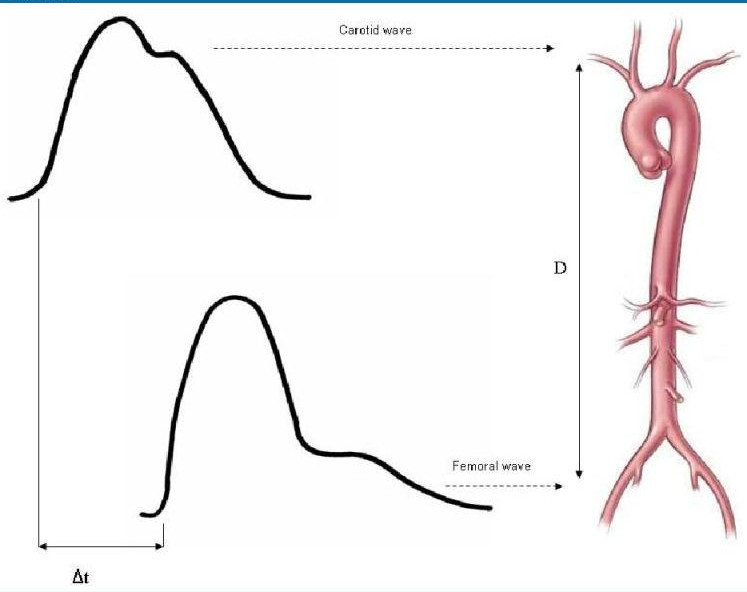
\includegraphics[width=\textwidth]{./Figures/VOP.jpg}
		{\footnotesize 	\textit{La medición de VOP se realiza a partir de dos mediciones de la curva de presión, con un desfasaje temporal conocido.} \par}		
	\end{minipage}
	\caption{Esquema de medición de VOP}
	\label{fig:vop}
\end{figure}

El dispositivo desarrollado en este trabajo está orientado a ser utilizado por investigadores médicos, ingenieros biomédicos, biólogos y veterinarios en grupos de trabajo en general aplicado a cardiología. En particular este trabajo se realiza para la Universidad Favaloro, y es importante porque permitirá avanzar a futuro en el conocimiento de formas de medición de presión ambulatoria indirecta, más precisas y menos invasivas.

\subsection{Bases físicas de la medición}

De acuerdo a la Organización Mundial de la Salud, la presión sanguínea humana es medida de la presión que ejerce la sangre circulante sobre las paredes de los vasos sanguíneos \cite{who2015}. Esta onda de presión es originada por el latido del corazón y transmitida hacia todo el árbol arterial. La composición entre la onda incidente y la reflejada dan origen a la onda estacionaria de presión, cuyo máximo y mínimo dan origen a los valores característicos conocidos como \textbf{presion sistólica} y \textbf{presión diastólica}. Estos valores tienen una gran importancia en la clínica. En un adulto sano, estos valores son aproximadamente 120mmHg para la presión sistólica y 80mmHg para la presión diastólica. En la figura \ref{fig:periodopresion} puede observarse una forma de onda característica.

\begin{figure}[!htbp]
	\centering
	\begin{minipage}{0.65\textwidth}
		
\includegraphics[width=\textwidth]{./Figures/periodopresion.png}
	{\footnotesize \textit{	La forma de onda característica de la presión humana se puede caracterizar como una onda estacionaria conformada por una onda pulsátil incidente y una onda reflejada.}\par}		
	\end{minipage}
	
	\caption{Forma de onda característica de la presión humana}
	\label{fig:periodopresion}
\end{figure}


\subsection{Estado del arte}

La medición ambulatoria de presión arterial (MAPA) braquial durante 24 horas es un método ampliamente aceptado para predecir riesgo cardiovascular y mortalidad\citep{hansen2006} \citep{staensen1999} \citep{verdecchia1993}. Se sabe que la variabilidad de la presión arterial y su pulsatilidad son el resultado de una compleja interacción entre el corazón y la red vascular. En particular, y para la evaluación de las características biomecánicas de la red arterial, se utiliza la velocidad de onda de pulso (VOP) como indicador indirecto de rigidez arterial \citep{nichols2008}.

Actualmente, existen diferentes técnicas para la medición de presión \citep{ogedegbe2010}. Pueden agruparse entre los métodos que brindan mediciones puntuales (presión sistólica, diastólica y media) y los que brindan mediciones contínuas. Entre los que brindan mediciones puntuales están el método auscultatorio, el método oscilométrico, método palpatorio, técnicas de ultrasonido, etc. Por otro lado, los que brindan mediciones contínuas suelen ser métodos invasivos como el catéter o no invasivos como la medición indirecta a partir de la medición de VOP \citep{ruso2001}.

La técnica más utilizada y difundida en la medicina clínica es el método oscilométrico, que basa su funcionamiento en monitorear las variaciones de la señal de presión en una banda inflable que se aplica alrededor del brazo izquierdo, logrando determinal a través del análisis de esta señal los valores de presión sistólica, diastólica y media de los pacientes. Mientras la banda se desinfla desde un nivel por encima de la presión sistólica, las paredes de la arteria comienzan a oscilar a medida que la sangre fluye a través del vaso parcialmente ocluído, y estas vibraciones son captadas en el transductor que monitorea la presión en la banda. Cuando la presión en la banda sigue disminuyendo, las oscilaciones aumentan hasta una amplitud máxima y luego disminuyen  hasta que la banda se desinfla completamente y el flujo de sangre regresa a la normalidad.

La presión en la banda en el punto de máxima oscilación normalmente se corresponde con la presión arterial media \ref{fig:moscilometrico}. El punto por encima de la presión media, en el cual las oscilaciones comienzan rápidamente a aumentar en amplitud se corresponde con la presión sistólica. El punto en que esta variación de las oscilaciones disminuye de forma más abrupta, se corresponde con la presión diastólica. Este método es de gran utilidad para la medicina clínica hace muchos años, sin embargo, tiene la contrapartida de que se pierde el detalle de la forma de onda de la curva de presión, lo cual es solo posible apreciar utilizando un sistema de adquisición contínuo con una tasa de muestreo adecuada.


\begin{figure}[!htbp]
	\centering
	\begin{minipage}{0.65\textwidth}
		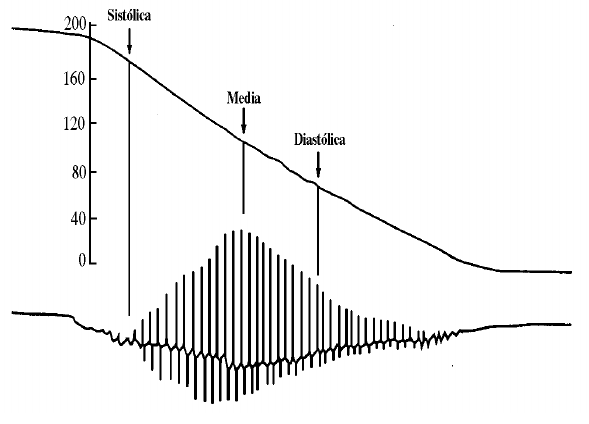
\includegraphics[width=\textwidth]{./Figures/moscilometrico.png}
		{\footnotesize \textit{La curva descendente corresponde a la presión de inflado de la almohadilla, mientras que la 	curva pulsátil inferior corresponde a la diferencia entre la presión arterial y la ejercida por la almohadilla. Esta última es la medición que se realiza con el manómetro manual. Con ayuda de un estetoscopio, se pueden detectar los ruidos correspondientes a la presión sistólica y diastólica.}\par}		
	\end{minipage}	
	
	\caption{Curva de inflado de la almohadilla de método oscilométrico vs. presión diferencial y ruidos detectados.}
	\label{fig:moscilometrico}
\end{figure}

Es claro que la medición de la onda contínua aporta muchos más datos que la medición de puntos característicos de la curva. A partir de la onda completa, se pueden calcular diferentes parámetros que permiten modelizar el árbol arterial y predecir enfermedades como hipertensión, arteriosclerosis, rigidez arterial, etc \citep{saito2011}  \citep{figueroa2014}.


\subsection{Medicion ambulatoria de presión arterial}

Una de las técnicas para medición contínua de presión es la medición indirecta a partir del VOP. El método más aceptado para medir VOP en pacientes consiste en el registro simultáneo de señales de presión en carótida y femoral. Conociendo la distancia y el desfasaje temporal entre estas mediciones de presión, se puede estimar la VOP como su cociente. La medición de VOP ha ingresado en las últimas guías de recomendación europeas como indicadora (Clase IIa; Nivel de evidencia B) para la evaluación subclínica de daño en órganos en pacientes hipertensos. El interés clínico en esta medición ha llevado al desarrollo de numerosos dispositivos para medir VOP y cuyas características y limitaciones están siendo analizadas actualmente para hallar un estándar internacional \citep{laurent2006} Así como la MAPA braquial ha impulsado el desarrollo de dispositivos de registro y análisis cada vez más sofisticados, la posibilidad de realizar un registro ambulatorio de VOP genera nuevos campos de investigación, así como la necesidad de que existan nuevos dispositivos \citep{omboni2016}.


Existen otros metodos de estimacion de la MAPA, pero se generan numerosas controversias debido a la complejidad matemática de las estimaciones y al uso de modelos matemáticos  arteriales unificados que suponen ser válidos para todos los pacientes. 
La presión arterial humana responde a una curva que tiene un pico y un valle, y una forma de onda característica. De esta curva pueden calcularse toda una serie de parámetros que modelizan el arbol arterial. Sin embargo, el método más utilizado en la medicina clínica para estimar la presión arterial, el método oscilométrico, solo toma dos valores característicos de esta curva, el máximo y el mínimo, denominados presion sistólica y presión diastólica.

\section{Motivación y Aplicaciones del equipo}

En este contexto, el estudio ambulatorio de la VOP en animales grandes podría brindar nuevas oportunidades para validar diferentes algoritmos de cálculo. La adquisición invasiva de señales de presión en dos sitios alejados del sistema arterial y a una distancia conocida, permite mejorar el conocimiento actual sobre la VOP en distintas condiciones del animal.

Las experiencias realizadas con este equipo permitirán profundizar la investigación sobre la medición indirecta de presión ambulatoria a partir de la medición de VOP y las técnicas para su cálculo. La aplicación de esta técnica para la MAPA permitirá desarrollar a futuro equipos portátiles que puedan medir de manera continua la presión de un paciente, con más información, mejor resolución y más comodidad.

Las experiencias de medición de VOP se realizan sobre animales grandes concientes, como ovejas o cerdos. Estos animales se encuentran previamente instrumentados con sensores de presión intraarteriales en forma crónica y tienen un prolongado período de adaptación a la vida en un corral de un laboratorio de investigación y al trato con los veterinarios. En la figura \ref{fig:oveja} puede verse una fotografía de una oveja durante una experiencia real con un equipamiento antiguo. La correcta adaptación del animal a la vida en el corral del laboratorio es muy importante porque la presión arterial se ve severamente afectada por la comodidad y bienestar del animal. Por ejemplo, algunas de las líneas de investigación estudian justamente la diferencia de los valores medios de presión entre el período de vigilia y de sueño. Este tipo de experiencias sobre un animal en estado de alerta se hace totalmente imposible.


\begin{figure}[!htbp]
	\centering
	
	\begin{minipage}{0.65\textwidth}
		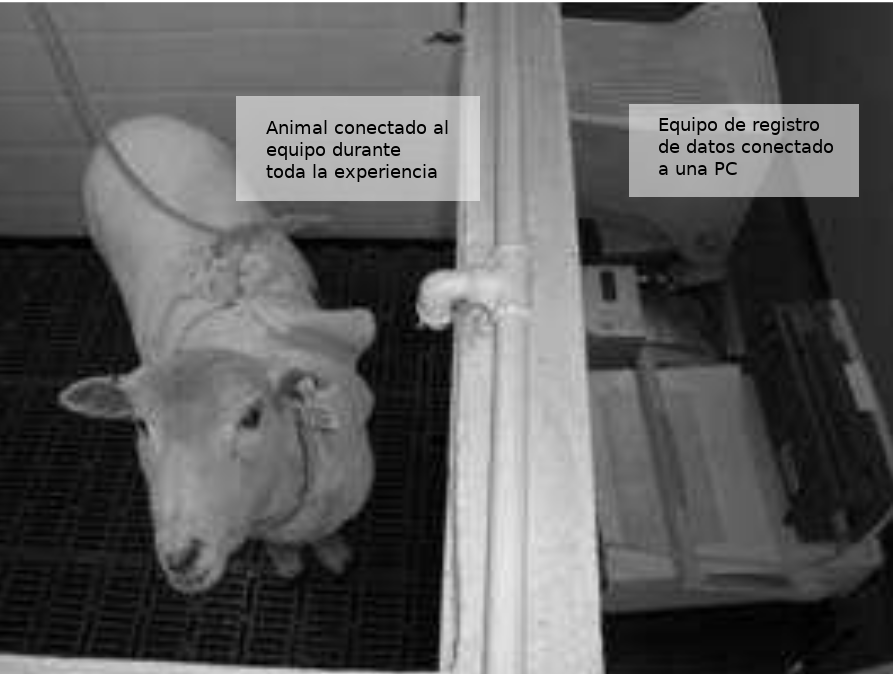
\includegraphics[width=\textwidth]{./Figures/oveja.png}
		{\footnotesize \textit{A la derecha se puede observar el equipo de registro de datos antiguo conectado a una PC y el animal conectado al equipo mediante un cable durante toda la experiencia}.\par}		
	\end{minipage}		
	
	\caption{Oveja instrumentada con un equipamiento antiguo con interfaz cableada.}
	\label{fig:oveja}
\end{figure}

El equipamiento de medición debe ir sobre el animal para evitar que existan cables que limiten el movimiento y dificulten la vida diaria del mismo. Además, luego de un período de adaptación, el equipo debe ser imperceptible para el animal. Esto se logra con un tamaño reducido, un sistema de carga cómoda, como una pequeña mochila, bajo peso, ausencia de ruido, etc. Durante toda la experiencia de medición, el equipo debe estar sobre el animal, y, en lo posible, solo debe acercarse personal de veterinaria para tareas de higiene y alimentación. El operador del equipo debería solamente acercarse al animal para la instalación del equipo, y para retirarlo al finalizar la experiencia. El resto del tiempo, el operador debe tener una interacción mínima con el animal.


\section{Objetivos y alcance}

El proyecto incluyó el desarrollo completo de un dispositivo de medición y adquisición de dos sensores de presión intraarteriales para ser utilizado en animales grandes, junto con su documentación técnica y manual de usuario. 

Las señales además se pueden visualizar en tiempo real para realizar algún eventual ajuste sobre el animal instrumentado antes de comenzar la experiencia. Este software de visualización no se incluye entre los alcances del proyecto, por lo que se utiliza solamente una interfaz en desarrollo a modo de prueba. 

El equipo se diseñó para ser portátil, alimentado por batería, con una autonomía aproximada de 24 horas. A la vez, se hizo énfasis en lograr un bajo peso que no moleste al animal durante la experiencia. La interfaz de carga es a través de la misma conexión USB.

El desarrollo del proyecto no incluye la fabricación del gabinete final ni del soporte para ser llevado por el animal. Tampoco se incluye el software de la terminal de configuración, solamente una versión preliminar para pruebas.

%----------------------------------------------------------------------------------------
